\chapter{Design and Implementation} \label{methode}
In this chapter, we will present our implementation of the SpMV over boolean semirings, how we implemented with HLS and how we connected the component in the FPGA.

\section{IP-core}
For this project, we have implemented an IP-core with Vivado HLS. The IP-core applies a modified version of SpMV over a adjacency matrix and a set of vertices known as seed nodes. We will have a brief introduction to HLS programming and how to customize the algorithm for HLS.

\subsection{IP-core}
Our implementation of the SpMV is done in HLS. Our algorithm takes in an adjacency matrix and a set of seed nodes as input, and outputs a result vector showing which node was activated after either all nodes are activated, or no more node can be. Unlike normal SpMV, where each iteration will activate all their neighbours, an ICM is dependent on a RNG and global or local probability. For this project, a global probability of 5\% was used. Each node have a 5\% chance to be activated, e.g. if $v_1$ was not activated by $V_r$ on the first iteration, $V_r$ can not reactivate $v_1$ on the next iteration. 

To prevent a reactivation as mentioned above. For each iteration, a frontier vector will be send in instead of the result from previous run as mentioned in Seciton \ref{BFS as Matrix}. A vector is a list of vertices. The frontier vector is generated by comparing the result from this run with a list of activated vertices. The vertices that was not on the list of activated node would be new activated vertices and would be the frontier. 

Our algorithm applies SpMV over the matrix and the frontier. For each iteration, each element in a row of the matrix is applied an AND (\&\&) operations with the corresponding element in the frontier vector. The resulting bit will be applied a OR ($\|$) operation between the other :
\begin{algorithm}
\begin{algorithmic}[2]
\State{(martix\_row[0] \&\& frontier[0])$\|$(matrix\_row[1] \&\& frontier[1])$\| \ldots$\\
(matrix\_row[n] \&\& frontier[n])$=$result[row]}
\end{algorithmic}
\end{algorithm}


Unlike the breadth first search on boolean semiring mentioned in earlier chapter, each node will have a chance to not be activated (set as '1'), even if matrix\_row[x] and frontier[x] = 1. This resulted that for each \&\&- operation, we need to \&\& another \textit{coin toss}, which determined if the activation takes place. The coin-toss is determined by the RNG and the global probability. 

The algorithm will continue until either all of the nodes are activated, or no more node can be activated. This is solved with the dist\_gen() function as we mention [INSERT PSEUDOCODE]. The function stops the algorithm when either frontier is empty (all the nodes are 0), or y (result) is full (all nodes = 1). 

In HLS the implementation of the ICM-SpMV was done in two level. The top level was the TopLevelWrapper. The TopLevelWrapper was set as the main function in our HLS implementation. The function takes in the address to the location to the matrix, the address to the result, and the address frontier. Since we are working with ICM, a global probability, a random seed as the initial state for the LFSR is also set as input. TopLevelWrapper stores the useful data over on local buffer, where it is sent to the datapth-function. The datapath-function is a sparse martix vector multiplication. 

The address to matrix, result,frontier, and the random seed and global probability is all mapped as AXI4-Lite while the matrix, frontier and the result are memory mapped. This allows us to send in the address of the memory location where the variables are stored and apply our algorithm. 
 
Since ICM is dependent on a random function, we ran each sets of seed nodes 50 times to find the average runtime and coverage to find the most optimal set of nodes.

\section{Linear-Feedback Shift Register}
The LFSR is a commonly used pseudo random number generator(RNG)\citep{murase1992linear}. Different sized LFRS is able to generate a wider range of pseudo random number. LFSR generates a pseudorandom number based on the previous number. The LFSR implemented for this project, is a 16 bit LFSR, the shift register is able to generate a pseudorandom number in the range from 0-$2^{16}(65536)$. We take the bit from position: 16,14,13 and 11, and XOR all the bits. resulting in (((16 XOR 14) XOR 13 ) XOR 11)=bit. The bit is pushed into bit-position 1 and the entire registers shifts towards right 1 bit. 
This allows the IP-core to generate a pseudo random number based on a initial seed input. From Figure: \ref{fig:LFSR} we can see that to continuously generate pseudo random numbers, the output from the LFSR is used as the next iterations seed. 

\begin{figure} 

\includegraphics[scale=0.3]{Figures/placeholder}
\caption{16-bit Linear-Feedback Shift Register}
	\label{fig:LFSR}
\end{figure}


\section{Design flow of HLS}
For this project, Xilinx Vivado HLS 2016.1 was used. The usual workflow in designing with Vivado HLS is as follow. 
\begin{enumerate}
\item Define your funciton/algorithm.
\item Simulate as compile code. 
\item Synthesise.
\item Co-simulate.
\end{enumerate}

The first step in designing with Vivado HLS is to define the algorithm that will be synthesise, for this report, its the matrix vector multiplication. After identifying different requirement and dependency, the algorithm is implemented in C with Vivado HLS. Vivado HLS have some limitation regarding the implementations:
\begin{itemize}
\item No dynamic memory (Need to be static), Vivado HLS does not support malloc, free, new or delete. 
\item NO STD, FILE-IO, etc, (no system calls). 
\item avoid recursive functions. 
\end{itemize}

The next step is to \textit{run C simulation}. This will verify that the C implementation is correct, the test in the testbench are created by the designer. After verifying that the implementation is correct, next step is to synthesise the implementation. Vivado HLS will then generate the appropriate Verolog or VHDL, depending on what the designer require. The finished generated solution is then reviewed. Vivado displays the "Synthesis Report", containing crucial information regarding the generated solution. There we can find the performance estimates of the generated core, the utilization estimates, and the interface to the generated core. After all this is done, Vivado offers a \textit{run C/RTL Cosimulation}. Vivado will then run both the C simulation and testbench, and the same testbench on a simulated version of the implemented core. This function allows the designer to verify that the generated core have the same behaviour as the simulated C implementation.

After Cosimulation is done, the IP-core is ready for export, \textit{Export RTL} generates the necessary RTL files and export the IP core. The exported IP-core can be found in the project folder and ready to be implement to the FPGA. 

There are some steps that Vivado HLS requires before the project can start. In the begining, Vivado HLS would require the designer to specify which function is the top level of the implementation. That top function would determine which port the IP core would have and what type of AXI4 protocol to implement. Vivado HLS also enables the user to specify to which platform this implementation is for.

The input and output port of the IP core is determined by the variables that functions require. Inputs that is read from, will automatically set as input, while variable that is only written to, will be set as output. Another thing about output is that for the core to understand that this is something that changes, it is often set as a pointer (For C code).VIVADO HLS generates control signal automatically. 

\section{Network and graph generator}
For this project, we choose to implement a R-mat generator as mentioned in Chapter: \ref{rmat} and  \cite{Rmat2004}. The generator is implemented in \textit{Python} \cite{PYTHON} with \textit{numpy}. The generator generates adjacency matrix with $2^k$ nodes, where \textit{k} is known as the scale of the sparse matrix. The total amount of edges the graph contains, is set as $total amoungt of edge = k \times edge factor $. The edge factor is the ratio of the graph's edge count to its vertex count\cite{graph500}. Our adjacency matrix was stored as a .txt format and was read as input for our IP core. 
We used the following variables to generate our adjacency matrix:
\begin{itemize}
\item \textbf{A} = 0.57
\item \textbf{B} = 0.19
\item \textbf{C} = 0.19
\item \textbf{D} = 1-0.57-0.19-0.19 = 0.05
\item \textbf{Edge factor}  = 16
\item \textbf{k (Scale)} =  10
\end{itemize}

By using the random-function provided by Python, we placed '1' in it's correct place. After the matrix is generated, we further applied a diagonal copying as shown in Figure:\ref{fig:flipDiagonal}. This is obligatory to generate an undirected graph.

For this project, a graph with size 1024 was used. This is a microscopic graph compared to graphs used in network analysis. 

\begin{figure}
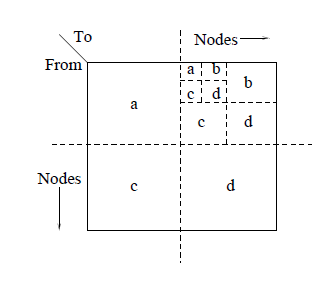
\includegraphics{Figures/Rmat}
\caption{The R-mat model \cite{Rmat2004}}
\label{fig:Rmat}
\end{figure}



\section{How is it connected}
To connect the IP core, we will use Xilinx Vivado (2016.1). In \textit{Block design}, we connected our xutom IP-Core to a 	\textit{ZYNQ7 processing system}\citep{FPGASoCManual}. The Zynq7 Processing system act as our PS, while the custom IP core act as our PL. The custop IP-core was connected to one of the High performance slave interface. For our implementation, the RNG was included with the core. This allows that 

For our core, we used the architecture of memory mapped. We pass the address in the form of AXI4-lite. The core includes an dma-function, which the HLS would initiate for us. This allows us to utilize the High performance slave interface.

%%INCLUDE A PICTURE TO ILLUSTRATE OUR POINT

\section{Xilinx SDK}
Vivado offers a \textit{Eclipse} based software develop kit (SDK). There we read the pregenerated graph from a SD card on the ZedBoard. We initiated the the custom IP core by setting all the required input signals.



\section{Optimization}
The function matrix\_vector\_multiplication() performes a single matrix vector multiplication. From the pseudocode, we can see that there is a room for parallization of the SpMV. The outer for loop from the pseudocode, can be parlized since the for loop is not dependent on the variable from the inner for-loop. 

Another paralization is during the simulation, after the spmv, the frontier needs to be calculated. And a converged() function is called in the end to determen if the simulation is finished. The frontier calculation and converged can pe run in parallel. 

include the different directives, PIPLINE

THe IP-core (currently) is only using around 2\% of the resource available on the FPGA(Zedboard). This gives us a lot of room for parallization of different core. Implemented 2 bus, one for input stream, one for output stream. The output stream consist of the result\_vector




\section{Potential improvement}:
For the second option, where the RNG core is not implemented into the IP CORE, we would have to have teh random number set as AXI4 stream from the buffer, since we would need to call a stream of random number from the core.


\section{global vs local probability}
For this project, a global activation chance was implemented, giving each node the same probability to be activated. A interesting model would be there are a personal probability of activation. Each node might have unique activation chance. Our implementation. 
